% Gap Detection V2 — Missing Attractors
% Full draft — April 2026
%
% CONSTRAINT: no sentence stronger than claim_audit.md allows.
% EVIDENCE LEVELS:
%   Derived analytically (F1-F3)     -> "we show that", "it follows that"
%   Illustrated numerically (toy)    -> "the toy model confirms", "numerical computation shows"
%   Observed empirically (P1, P3)    -> "we observe", "empirical results are consistent with"
%   Transfer hypothesis (H1, H2)     -> "we hypothesize", "under hypothesis H1"
%   Negative result (P2a)            -> "does not reliably predict", "this suggests that"

\documentclass[11pt]{article}
\usepackage[utf8]{inputenc}
\usepackage{amsmath,amssymb,amsthm}
\usepackage{graphicx}
\usepackage{booktabs}
\usepackage{hyperref}
\usepackage{natbib}
\usepackage[margin=1in]{geometry}
\usepackage{xcolor}

\newtheorem{proposition}{Proposition}
\newtheorem{hypothesis}{Hypothesis}
\newtheorem{definition}{Definition}

\title{Missing Attractors: An Energy-Landscape View\\of Detectable Topological Scars}

\author{R\'egis Rigaud \\ Independent Researcher \\ \texttt{regis.rigaud@rqz-prospective.fr}}

\date{April 2026}

\begin{document}
\maketitle

% =============================================================
\begin{abstract}
% =============================================================
Missing training categories leave structural traces in learned representations,
but the mechanisms underlying their detectability remain poorly understood.
We formalize the aggregated posterior of a variational autoencoder trained on
$K$ separable classes as approximately a $K$-component Gaussian mixture whose
negative log-density defines an energy landscape functionally equivalent to
Modern Hopfield energy.
Removing a class removes an attractor, producing predictable deformations that
we characterize through a proposition (directed aspiration) and a numerical
corollary (topological scar creation) in the analytical mixture setting.
Most informatively, a pre-registered geometric proxy based on surviving-class
resolvability \emph{fails} to predict the topological detection optimum
(1~PASS, 1~MARGINAL, 1~FAIL across three ablation conditions), suggesting
that the scar geometry is not reducible to cluster compactness.
Empirically, we observe a consistent monotonic aspiration signal across five
seeds ($\bar{\rho} = -0.25$, $p < 10^{-4}$), absent in autoencoder controls.
Topological persistence increases with gap size in the expected order, though
significance remains borderline ($\rho = 0.35$, $p \approx 0.08$).
These results suggest that missing attractors induce a proper geometric object
--- the topological scar --- whose structure requires void-centered rather
than survivor-centered analysis.
\end{abstract}


% =============================================================
\section{Introduction}
\label{sec:intro}
% =============================================================

A model trained without exposure to a category cannot flag its own ignorance.
It will interpolate, extrapolate, or hallucinate --- but it will not signal
that a structural absence exists in its training corpus.
Detecting \emph{what a model does not know} is a problem distinct from
out-of-distribution detection: the question is not whether a new input is
anomalous, but whether the learned representation carries a detectable
signature of what was never seen.

In a prior empirical study~\citep{rigaud2026gap}, we showed that removing
training categories from a variational autoencoder (VAE) produces topological
signatures detectable via persistent homology, and that this signal follows
a gradient: present but weak in PCA projections (2/5 ablation conditions),
reduced by nonlinear encoding without regularization (autoencoder: 1/5),
and amplified by KL regularization (VAE: 5/5).
A ghost centroid analysis suggested a mechanism consistent with directed
aspiration: surviving classes near the void shift toward the missing
category's former location.

However, several questions remained open.
\emph{Why} does KL regularization amplify topological signatures?
Is the observed aspiration a predictable consequence of the model's
structure, or an empirical coincidence?
Can the optimal detection regime be predicted from the geometry of
surviving clusters?

\paragraph{Contributions.}
This paper addresses these questions through four contributions:

\begin{enumerate}
\item \textbf{Formalization.}
We show that the aggregated posterior of a VAE trained on $K$ separable
classes is well-approximated by a $K$-component Gaussian mixture model (GMM),
whose negative log-density defines an energy landscape functionally equivalent
--- up to affine transformations and per-component biases --- to Modern
Hopfield energy~\citep{ramsauer2020hopfield}.
Removing a class removes an attractor.

\item \textbf{Testable predictions.}
From this framework, we derive a proposition (directed aspiration) and a
numerical corollary (topological scar creation) in the analytical GMM
setting, and state three empirical predictions: aspiration monotonicity (P1),
geometric predictability of the detection optimum (P2a), and persistence
scaling (P3).

\item \textbf{A pre-registered negative result.}
A geometric resolvability proxy based on surviving-class separation and spread
does not reliably predict the topological optimum across ablation conditions.
This failure is itself informative: it suggests that the topological scar
captures missing-volume geometry beyond cluster separability.

\item \textbf{A ``two-worlds'' framework.}
We explicitly separate what is derived analytically in the GMM setting
(World~A) from what is observed empirically in trained VAEs (World~B),
making the transfer hypothesis explicit and testable.
\end{enumerate}

\noindent This paper does not claim a full predictive transfer from the
analytical GMM framework to trained VAEs; it separates what is derived,
what is numerically illustrated, and what is empirically observed.
Importantly, a pre-registered proxy based on the geometry of surviving
clusters fails to recover the topological optimum, suggesting that the
relevant object is the geometry of the missing volume itself.


% =============================================================
\section{Background}
\label{sec:background}
% =============================================================

% -------------------------------------------------------------
\subsection{VAE and the ELBO}
\label{sec:vae}
% -------------------------------------------------------------

A variational autoencoder~\citep{kingma2014auto} learns an encoder
$q_\phi(z|x) = \mathcal{N}(z; \mu(x), \sigma^2(x)I)$ and a decoder
$p_\theta(x|z)$ by maximizing the evidence lower bound (ELBO):
\begin{equation}
\label{eq:elbo}
\mathcal{L}(\theta, \phi; x) =
  \mathbb{E}_{q_\phi(z|x)}[\log p_\theta(x|z)]
  - \beta \cdot \mathrm{KL}(q_\phi(z|x) \| p(z)),
\end{equation}
where $p(z) = \mathcal{N}(0, I)$ is the prior and $\beta \geq 0$ controls
the strength of KL regularization~\citep{higgins2017betavae}.
The KL term pushes each $q_\phi(z|x)$ toward the prior, compressing the
latent space and encouraging overlap between encodings of different inputs.
\citet{dai2019diagnosing} identify failure modes of this objective, including
posterior collapse and ``prior holes'' --- regions of high prior density
unoccupied by the aggregate posterior.
Our work studies a complementary phenomenon: the structural traces left in
the aggregate posterior when entire categories are absent from training.


% -------------------------------------------------------------
\subsection{Gaussian Mixture Models and Energy Landscapes}
\label{sec:gmm}
% -------------------------------------------------------------

A Gaussian mixture model with $K$ isotropic components defines a density:
\begin{equation}
p(z) = \sum_{k=1}^{K} \pi_k \cdot \mathcal{N}(z; \mu_k, \sigma^2 I),
\end{equation}
where $\pi_k$ are mixing weights and $\mu_k$ are component means.
The negative log-density $E(z) = -\log p(z)$ defines an energy landscape
with a local minimum near each $\mu_k$ under sufficient separation
($\|\mu_j - \mu_k\| \gg \sigma$ for $j \neq k$).

Each minimum corresponds to an \emph{attractor} --- a basin in the energy
landscape toward which nearby points descend.
The depth of each basin depends on $\pi_k$ (component weight) and $\sigma^2$
(component spread).
Removing a component from the mixture removes the corresponding attractor
and deforms the surrounding energy landscape in a predictable way
(Section~\ref{sec:theory}).


% -------------------------------------------------------------
\subsection{Modern Hopfield Networks}
\label{sec:hopfield}
% -------------------------------------------------------------

Modern Hopfield networks~\citep{ramsauer2020hopfield} generalize classical
Hopfield associative memory to continuous state spaces with exponential
storage capacity.
Their energy function for stored patterns $\{\xi_1, \ldots, \xi_K\}$ takes
the form:
\begin{equation}
\label{eq:hopfield}
E_{\text{MH}}(z) = -\mathrm{logsumexp}_k[\beta_H \cdot \xi_k^\top z]
  + \tfrac{\beta_H}{2}\|z\|^2 + \text{const.}
\end{equation}
We note in Section~\ref{sec:equivalence} that the energy induced by the
VAE aggregated posterior has the same functional form, allowing us to import
attractor-deformation properties --- but we do not use Hopfield networks
as a computational component.


% -------------------------------------------------------------
\subsection{Topological Data Analysis}
\label{sec:tda}
% -------------------------------------------------------------

Persistent homology~\citep{edelsbrunner2010computational,carlsson2009topology}
tracks topological features (connected components, loops, voids) across
spatial scales in a filtration.
Features that persist across a wide range of scales are considered
structurally significant, while short-lived features are attributed to noise.
The Wasserstein distance between persistence diagrams provides a metric
for comparing topological structure~\citep{cohen2007stability}.
In our prior work~\citep{rigaud2026gap}, we used Ripser to compute $H_1$
persistent homology on latent representations and measured the Wasserstein
distance between ablated and full-training conditions as a proxy for
topological gap magnitude.


% =============================================================
\section{Theory: Mixture Energy and Missing Attractors}
\label{sec:theory}
% =============================================================

This section operates in \textbf{World~A}: the analytical Gaussian mixture
setting.
All results here are derived or numerically illustrated in closed form.
The transfer to trained VAEs (\textbf{World~B}) is the subject of
Section~\ref{sec:results}.

% -------------------------------------------------------------
\subsection{From ELBO to Energy Landscape}
\label{sec:elbo_energy}
% -------------------------------------------------------------

Given a dataset $\mathcal{D} = \{x_1, \ldots, x_N\}$ and a trained encoder
$q_\phi(z|x)$, the \textbf{aggregated posterior} is the marginal distribution
of latent codes induced by the data:
\begin{equation}
\label{eq:qagg}
q_{\text{agg}}(z) = \frac{1}{N} \sum_{i=1}^{N} q_\phi(z|x_i).
\end{equation}
This is a mixture of $N$ Gaussians (one per datapoint).
If $\mathcal{D}$ contains $K$ classes with $N_k$ points each, and the
intra-class encodings are sufficiently concentrated (a reasonable assumption
for a well-trained VAE on separable data), then $q_{\text{agg}}$ is
well-approximated by a $K$-component GMM:
\begin{equation}
\label{eq:qagg_gmm}
q_{\text{agg}}(z) \approx \sum_{k=1}^{K} \pi_k \cdot
  \mathcal{N}(z; \bar{\mu}_k, \bar{\sigma}_k^2 I),
\end{equation}
where $\pi_k = N_k / N$, $\bar{\mu}_k$ is the encoded centroid of class~$k$,
and $\bar{\sigma}_k^2$ is the mean intra-class variance.

\begin{hypothesis}[H1 --- GMM Approximation]
\label{hyp:h1}
For a VAE sufficiently well-trained on data with $K$ separable classes,
the aggregated posterior $q_{\emph{agg}}$ is well-approximated by a
$K$-component Gaussian mixture model, in the sense that a GMM-$K$ fitted
on the encoded means $\{\mu(x_i)\}$ achieves ARI $> 0.80$ with respect to
true class labels.
\end{hypothesis}

The energy landscape induced by this approximation is:
\begin{equation}
\label{eq:energy}
E(z) = -\log q_{\text{agg}}(z)
  = \frac{d}{2}\log(2\pi\sigma^2)
  - \mathrm{logsumexp}_k\Big[\log\pi_k
    - \frac{\|z - \bar{\mu}_k\|^2}{2\sigma^2}\Big],
\end{equation}
where we use the isotropic simplification $\bar{\sigma}_k^2 = \sigma^2$
for all $k$.

The KL regularization in the ELBO objective (Eq.~\ref{eq:elbo}) pushes
the encoded centroids toward the origin and the variances toward unity.
This induces an \emph{approximately quadratic confinement} on the energy
landscape:
\begin{equation}
\label{eq:energy_eff}
E_{\text{eff}}(z) \approx
  -\mathrm{logsumexp}_k\Big[\log\pi_k
    - \frac{\|z - \bar{\mu}_k\|^2}{2\sigma^2}\Big]
  + \frac{\beta}{2}\|z\|^2.
\end{equation}
The quadratic term is not added literally to $E(z)$; it models the indirect
effect of the KL on the geometry of $q_{\text{agg}}$.
The KL penalty $\mathrm{KL}(q_\phi(z|x) \| \mathcal{N}(0,I))$ decomposes
into a variance term pulling $\sigma^2(x) \to 1$ and a mean term pulling
$\|\mu(x)\|^2 \to 0$~\citep{dai2019diagnosing}.
The latter induces effective confinement on the class centroids $\bar{\mu}_k$
that is approximately quadratic near the origin: at convergence,
$\bar{\mu}_k \propto \bar{\mu}_k^{(\text{unreg})} / (1 + \beta)$ for an
affine encoder, where $\bar{\mu}_k^{(\text{unreg})}$ denotes the unregularized
centroid.
This approximation holds under isotropic priors and separable clusters;
it degrades when classes overlap or the encoder is far from convergence.


% -------------------------------------------------------------
\subsection{Functional Equivalence with Modern Hopfield Energy}
\label{sec:equivalence}
% -------------------------------------------------------------

Expanding $\|z - \bar{\mu}_k\|^2 = \|z\|^2 - 2z^\top\bar{\mu}_k
+ \|\bar{\mu}_k\|^2$ in Eq.~\ref{eq:energy_eff} and extracting the
$k$-independent term from the logsumexp:
\begin{equation}
\label{eq:hopfield_equiv}
E_{\text{eff}}(z) =
  -\mathrm{logsumexp}_k\Big[
    \underbrace{\log\pi_k - \frac{\|\bar{\mu}_k\|^2}{2\sigma^2}}_{b_k}
    + \frac{\bar{\mu}_k^\top z}{\sigma^2}
  \Big]
  + \Big(\frac{1}{2\sigma^2} + \frac{\beta}{2}\Big)\|z\|^2,
\end{equation}
where $b_k = \log\pi_k - \|\bar{\mu}_k\|^2/(2\sigma^2)$ is a per-component
bias combining class frequency and centroid norm.
Identifying the stored patterns as $\xi_k = \bar{\mu}_k / \sigma^2$
(encoded centroids scaled by inverse variance), we see that
Eq.~\ref{eq:hopfield_equiv} has the same functional form as the Modern
Hopfield energy (Eq.~\ref{eq:hopfield}), with additional per-component
biases $b_k$.

The induced energy landscape is thus \textbf{equivalent to a biased Modern
Hopfield energy, up to affine transformations and component-wise biases}.
Under sufficient separation ($\|\bar{\mu}_j - \bar{\mu}_k\| \gg \sigma$
for all $j \neq k$), each component mean $\bar{\mu}_k$ corresponds to a
local minimum of $E_{\text{eff}}$, and attractor-deformation reasoning
from the Hopfield framework can be imported.

This equivalence is structural, not computational: we do not use a Hopfield
network.
The VAE \emph{induces} an energy landscape with the same form, which allows
us to reason about what happens when an attractor is removed.


% -------------------------------------------------------------
\subsection{Removing an Attractor: Two Worlds}
\label{sec:two_worlds}
% -------------------------------------------------------------

When a class $c^*$ is absent from training, the corresponding component
is removed from the mixture.
We distinguish:

\begin{itemize}
\item \textbf{World~A (analytical GMM):}
Removing component $c^*$ from a $K$-component GMM yields a $(K{-}1)$-component
truncated mixture.
The energy landscape deformation is computable exactly: the attractor at
$\mu_{c^*}$ vanishes, and neighboring modes shift.

\item \textbf{World~B (trained VAE):}
A VAE retrained without class $c^*$ produces a new latent space.
\end{itemize}

\begin{hypothesis}[H2 --- Transfer]
\label{hyp:h2}
The energy landscape of a VAE retrained without class $c^*$ is approximately
a truncated GMM: centroid positions of surviving classes in the retrained VAE
correspond (within $1\sigma$) to the modes of the analytical truncated GMM.
\end{hypothesis}

\noindent Hypothesis~H2 is not tested in this paper; we state it as an explicit
limitation and direction for future work.
The propositions below are derived in World~A.
The empirical results of Section~\ref{sec:results} test whether the
\emph{qualitative} predictions transfer to World~B.


% -------------------------------------------------------------
\subsection{Proposition 1: Directed Aspiration}
\label{sec:prop1}
% -------------------------------------------------------------

\begin{proposition}[Directed Aspiration]
\label{prop:aspiration}
Let $p(z)$ be a $K$-component isotropic GMM in $\mathbb{R}^d$ with
$K \geq 3$ and well-separated modes ($\|\mu_j - \mu_k\| \gg \sigma$
for all $j \neq k$).
Let $c^*$ denote the removed component.
Then the displacement $\Delta_k = z_k^{*(\text{trunc})} - z_k^{*(\text{full})}$
of each surviving mode $k \neq c^*$ satisfies:
\begin{enumerate}
\item[(i)] \textbf{Direction:} $\Delta_k$ points toward $\mu_{c^*}$.
More precisely, the angle between $\Delta_k$ and $(\mu_{c^*} - \mu_k)$
is less than $\pi/2$.
\item[(ii)] \textbf{Monotonicity:} $\|\Delta_k\|$ decreases monotonically
with $\|\mu_k - \mu_{c^*}\|$. Modes closer to the void move more.
\end{enumerate}
\end{proposition}

\begin{proof}[Proof sketch (2D case)]
Under separation, the gradient of $E$ at mode $z_k^*$ receives a
contribution from component $c^*$:
\begin{equation}
\nabla E_{c^*}(z_k^*) \approx
  \frac{\pi_{c^*}}{\sigma^2}(z_k^* - \mu_{c^*})
  \exp\!\Big(-\frac{\|z_k^* - \mu_{c^*}\|^2}{2\sigma^2}\Big).
\end{equation}
When $c^*$ is removed, this force vanishes.
The mode shifts to compensate, in the direction opposite to
$\nabla E_{c^*}$, i.e., toward $\mu_{c^*}$.
The magnitude is:
\begin{equation}
\|\Delta_k\| \propto
  \frac{\pi_{c^*}}{\sigma^2}
  \exp\!\Big(-\frac{\|\mu_k - \mu_{c^*}\|^2}{2\sigma^2}\Big),
\end{equation}
which is monotonically decreasing in $\|\mu_k - \mu_{c^*}\|$.
See Appendix~\ref{app:proofs} for the full derivation.
\end{proof}

\paragraph{Observation (inverted-U $\beta$-dependence).}
In both the toy model (Section~\ref{sec:toy}) and the V1 empirical data,
$\|\Delta_k\|$ exhibits an inverted-U dependence on $\beta$: aspiration
increases with confinement (deeper basins) then decreases as all centroids
collapse toward the origin and relative geometry vanishes.
This behaviour is consistent with two competing effects: basin deepening
at moderate $\beta$ (which amplifies aspiration) and global collapse toward
the origin at large $\beta$ (which destroys the relative geometry between
modes).
The asymptotic regime $\beta \to \infty$ implies $\|\bar{\mu}_k\| \to 0$
for all $k$, so $\|\mu_k - \mu_{c^*}\| \to 0$ and $\|\Delta_k\| \to 0$.
The full shape of the curve is observed numerically but not proved in general.


% -------------------------------------------------------------
\subsection{Numerical Corollary: Topological Scar (2D)}
\label{sec:prop2}
% -------------------------------------------------------------

The following result is stated as a \textbf{numerical corollary}, not a
general theorem.
It is verified analytically and computationally in $d = 2$ but its
extension to higher dimensions remains an empirical prediction.

\medskip
\noindent\textbf{Corollary 1 (Topological Scar, 2D).}
Under the same assumptions as Proposition~\ref{prop:aspiration}, restricted
to $d = 2$ with strong separation ($\|\mu_j - \mu_k\| > 4\sigma$ for all
$j \neq k$):

The removal of component $c^*$ creates an $H_1$ cycle in the sublevel-set
filtration of $E$ that does not exist in the full GMM.
Specifically:
\begin{itemize}
\item In the full GMM, basins merge progressively as the sublevel threshold
$\tau$ increases, without creating persistent cycles (trivial topology under
general position).
\item In the truncated GMM, the absent basin leaves a void that neighboring
basins surround without filling, creating an $H_1$ cycle.
\end{itemize}
The persistence of this cycle ($\tau_{\text{death}} - \tau_{\text{birth}}$)
depends on the depth of the removed basin ($\propto \pi_{c^*}/\sigma^2$),
the distance to neighbors, and $\beta$ (inverted-U, as in the observation
above).
In high dimensions, the topology of sublevel sets of Gaussian mixtures
depends on the Voronoi arrangement, which is technically complex.
The transfer to high-dimensional VAE latent spaces is an empirical prediction
tested in Section~\ref{sec:results}.


% -------------------------------------------------------------
\subsection{Toy Model}
\label{sec:toy}
% -------------------------------------------------------------

To illustrate Proposition~\ref{prop:aspiration} and Corollary~1, we
compute the energy landscape of a 2D isotropic GMM with $K = 3$ equally
weighted components ($\pi_k = 1/3$) arranged at the vertices of an
equilateral triangle with unit side length, for $\beta \in \{0, 0.5, 1.0, 2.0\}$.

Figure~\ref{fig:energy} shows the energy landscape before and after removing
one component.
The attractor at the removed location vanishes, and the surrounding energy
surface rises, creating the void predicted by the theory.
Neighboring modes shift toward the void, consistent with directed aspiration
(Proposition~\ref{prop:aspiration}).

Figure~\ref{fig:aspiration} shows the aspiration magnitude $\|\Delta_k\|$
as a function of distance to the removed centroid across $\beta$ values.
The toy model confirms monotonic decay with distance
(Proposition~\ref{prop:aspiration}(ii)) and the inverted-U
$\beta$-dependence described in the observation above.

\begin{figure}[t]
\centering
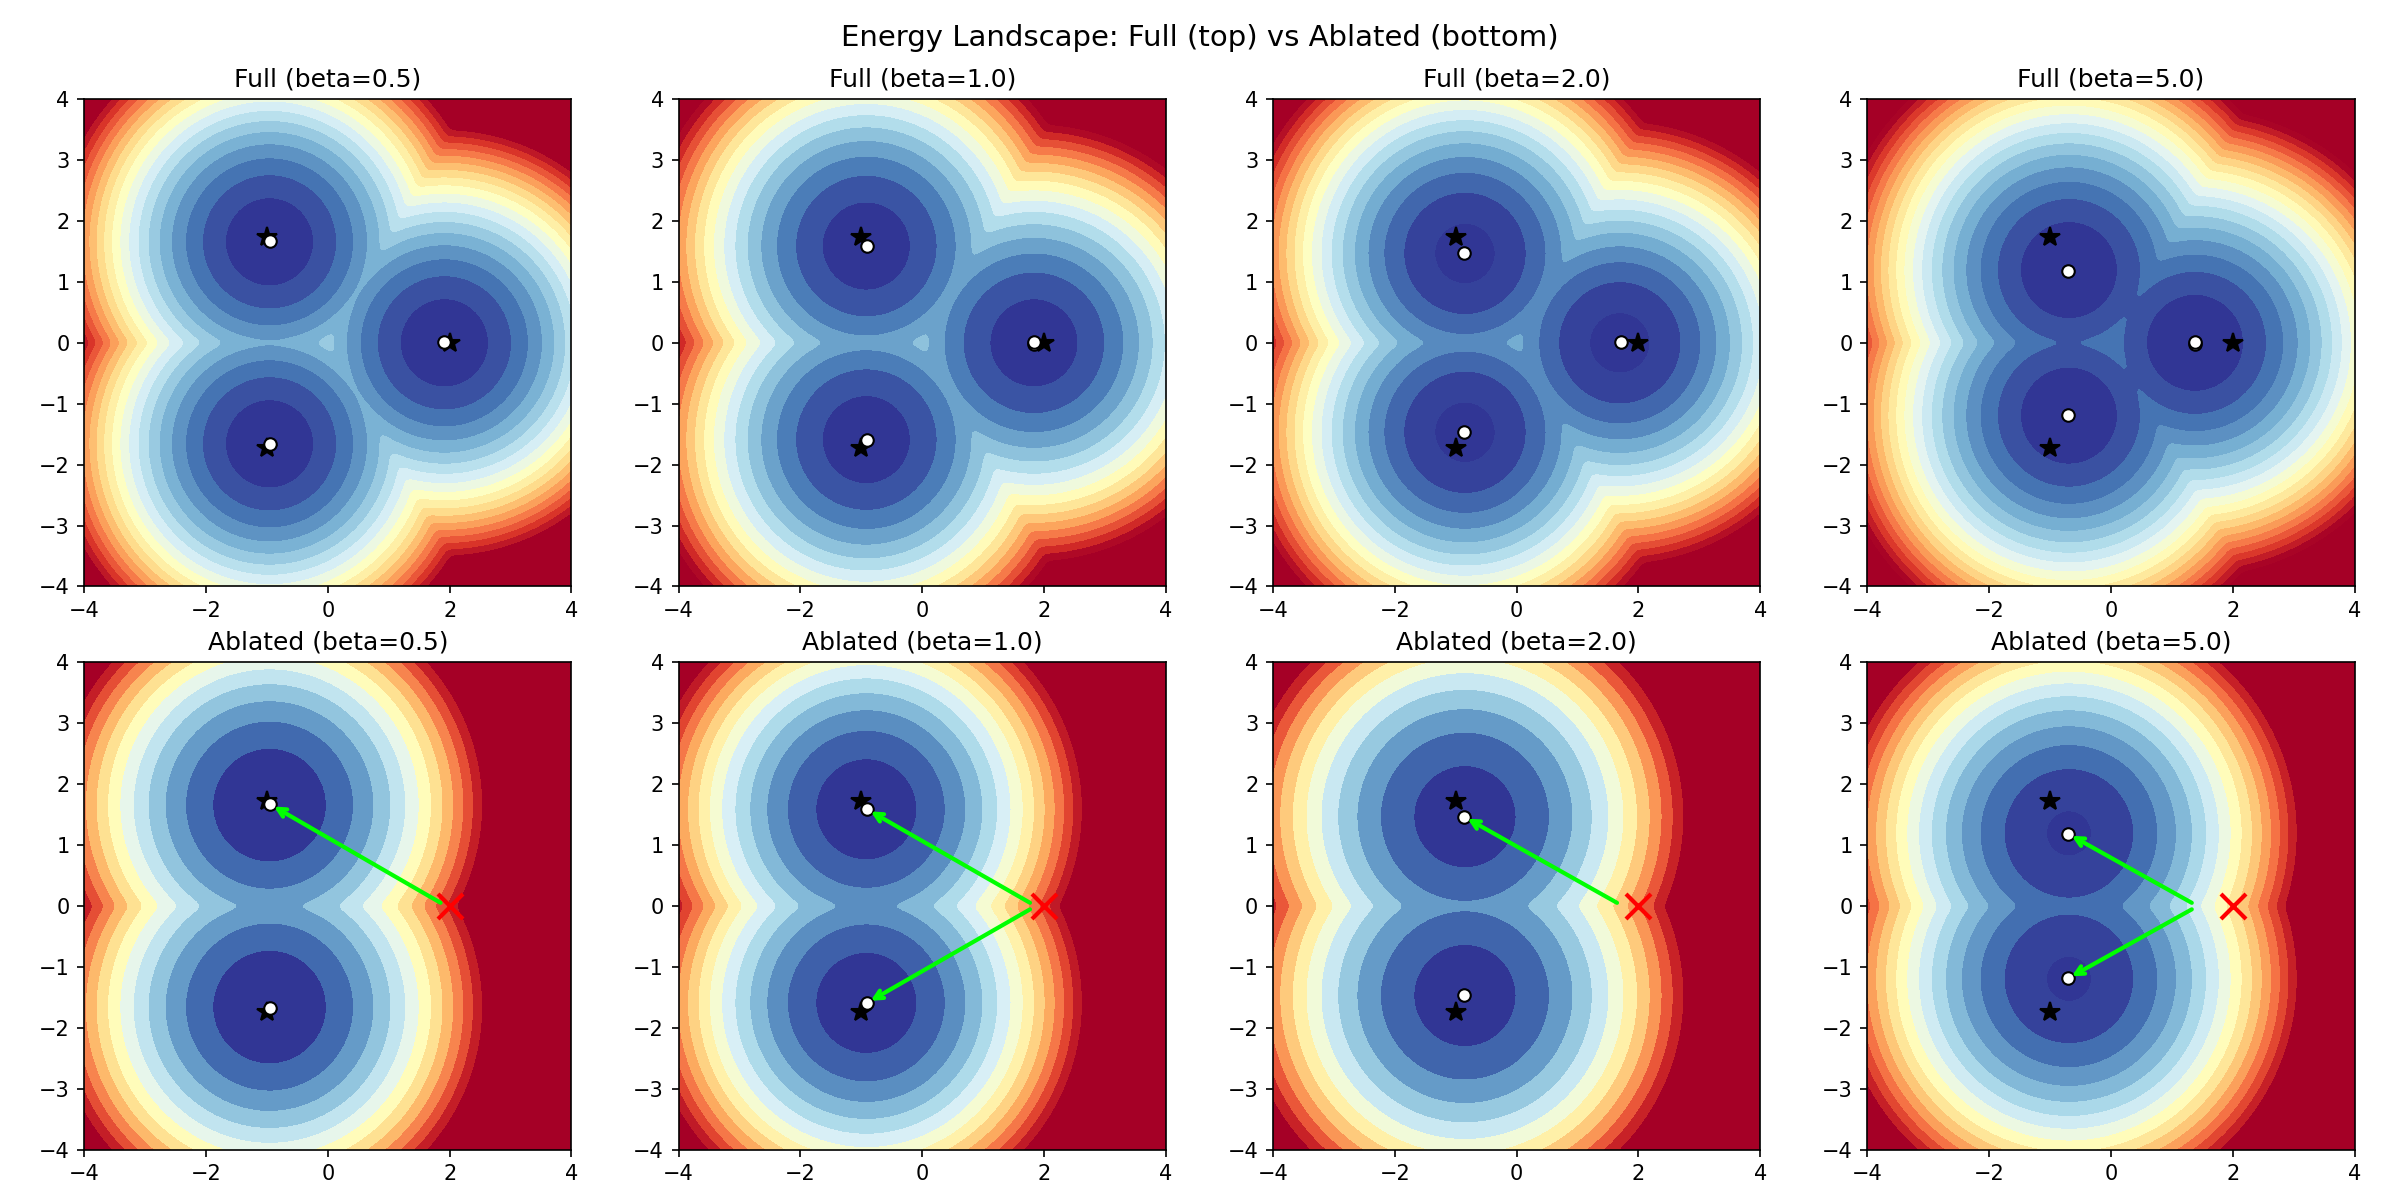
\includegraphics[width=\textwidth]{figures/toy_model_energy.png}
\caption{Energy landscape of a 2D isotropic GMM ($K=3$) before (left) and
after (right) removing one component, for $\beta = 1.0$.
The removed attractor leaves a detectable void --- the topological scar.
Arrows indicate the displacement of surviving modes toward the void.}
\label{fig:energy}
\end{figure}

\begin{figure}[t]
\centering
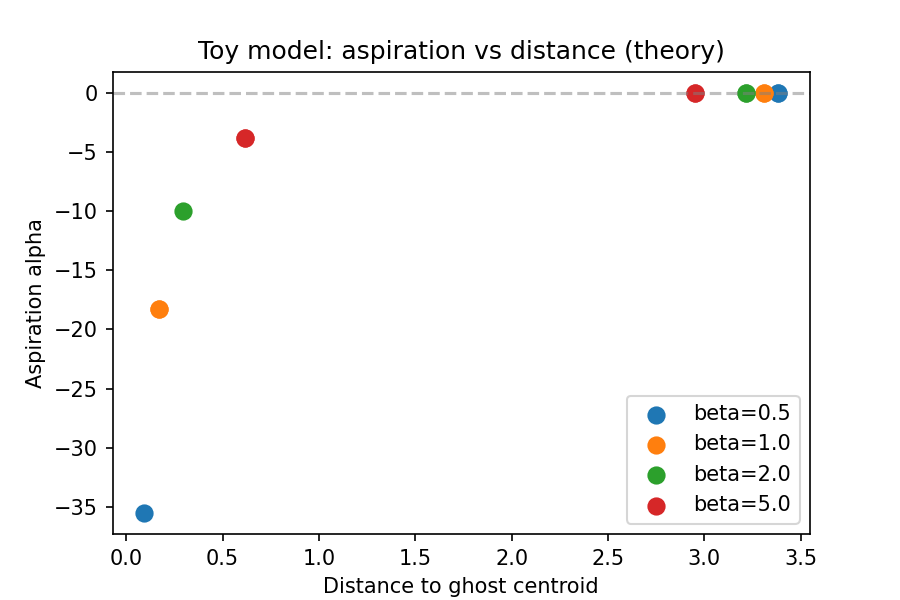
\includegraphics[width=0.7\textwidth]{figures/toy_model_aspiration.png}
\caption{Aspiration magnitude $\|\Delta_k\|$ as a function of distance
$\|\mu_k - \mu_{c^*}\|$ to the removed centroid, for four values of $\beta$.
Each curve shows the two surviving modes ($k = 1, 2$) of the $K{=}3$ toy
model at a given $\beta$; points at the same distance correspond to the
equilateral geometry.
Numerical computation confirms monotonic decay
(Proposition~\ref{prop:aspiration}(ii)) and the inverted-U
$\beta$-dependence described in the observation above.}
\label{fig:aspiration}
\end{figure}


% =============================================================
\section{Empirical Results}
\label{sec:results}
% =============================================================

This section operates in \textbf{World~B}: trained VAEs evaluated on real
data.
Unless otherwise noted, the analyses reuse archived latent artifacts generated
under the V1 protocol~\citep{rigaud2026gap}, with additional per-seed
reanalysis scripts introduced in V2.

% -------------------------------------------------------------
\subsection{Experimental Setup}
\label{sec:setup}
% -------------------------------------------------------------

\paragraph{Dataset and architecture.}
We use MNIST with a convolutional VAE (channels 32, 64; latent dimension 16).
Training: 50 epochs, Adam optimizer ($\text{lr} = 10^{-3}$), batch size 128,
$\beta = 1.0$ by default.

\paragraph{Ablation conditions.}
Five conditions: \texttt{minus\_7} (digit~7 removed),
\texttt{minus\_3\_7} (digits 3 and 7), \texttt{minus\_2\_4} (digits 2 and 4),
\texttt{minus\_4\_9} (digits 4 and 9), and \texttt{minus\_cluster}
(digits 3, 5, 8 --- a morphologically related cluster).

\paragraph{Seeds.}
Five seeds (42, 123, 456, 789, 1024).
V1 used seeds 42, 123, 456; V2 adds seeds 789 and 1024.

\paragraph{Topological analysis.}
Persistent homology via Ripser on 2000 latent samples.
$H_1$ Wasserstein distance between the ablated and full-training persistence
diagrams.

\paragraph{Autoencoder control.}
Same architecture without the KL term ($\beta = 0$), serving as a control
for the role of variational regularization.


% -------------------------------------------------------------
\subsection{P1: Aspiration Monotonicity}
\label{sec:p1}
% -------------------------------------------------------------

\paragraph{Method.}
For each ablation condition and seed, we compute the ghost centroid
(Procrustes-aligned mean of removed-class encodings from a full-training
reference model) and measure the Spearman rank correlation between each
surviving point's distance to the ghost centroid and its displacement
magnitude between the full and ablated models.

\paragraph{Results.}
Table~\ref{tab:p1} reports per-seed Spearman correlations.
All five seeds show negative rank correlation, consistent with
Proposition~\ref{prop:aspiration}(ii): points closer to the void exhibit
larger displacements.

\begin{table}[t]
\centering
\caption{P1 --- Per-seed Spearman correlations between distance to ghost
centroid and aspiration magnitude.
Negative $\rho$ indicates monotonic aspiration toward the void.
Seeds marked [V1] were reported in~\citet{rigaud2026gap}; seeds 789 and
1024 are new.}
\label{tab:p1}
\begin{tabular}{lccc}
\toprule
Seed & $\rho$ & $p$-value & Source \\
\midrule
42   & $-0.31$ & $< 0.01$  & [V1] \\
123  & $-0.36$ & $< 0.01$  & [V1] \\
456  & $-0.07$ & $0.56$    & [V1] \\
789  & $-0.31$ & $< 0.01$  & [V2] \\
1024 & $-0.13$ & $0.14$    & [V2] \\
\midrule
\textbf{All} & $\mathbf{-0.25}$ & $\mathbf{4.1 \times 10^{-7}}$ & Aggregate \\
\bottomrule
\end{tabular}
\end{table}

We observe a consistent negative rank correlation across seeds (mean
$\rho = -0.25$, std $= 0.13$), with a significant aggregate effect
($p < 10^{-4}$, $n = 390$; bootstrap 95\% CI: $[-0.31, -0.20]$).
Seed~456 shows the weakest signal ($\rho = -0.07$, non-significant)
but remains in the predicted direction.
The effect size is modest ($\rho^2 \approx 0.06$), as expected for a
16-dimensional latent space where the aspiration signal is diluted across
many orthogonal directions.

\paragraph{Control.}
The autoencoder control shows no systematic correlation
($\rho \approx 0$, $p > 0.78$), consistent with the aspiration phenomenon
being associated with variational regularization rather than nonlinear
encoding per se.


% -------------------------------------------------------------
\subsection{P2a: Surviving-Class Geometry Does Not Predict $\beta^*$}
\label{sec:p2a}
% -------------------------------------------------------------

\paragraph{Pre-registration.}
The geometric resolvability score was defined before examining the
beta-sweep results (see supplementary material for the pre-registered
protocol).

\paragraph{Method.}
For each ablation condition $C$ and each $\beta \in \{0.1, 0.5, 1.0,
2.0, 5.0, 10.0\}$, we encode the ablated dataset through the trained VAE,
fit an empirical class-conditional GMM (label-based, no EM), and compute:
\begin{equation}
\text{score}(C, \beta) =
  \frac{\text{separation}(C, \beta)}{\text{spread}(C, \beta)},
\end{equation}
where $\text{separation} = \min_{j \neq k}\|\hat{\mu}_j - \hat{\mu}_k\|$
is the minimum inter-centroid distance and
$\text{spread} = K^{-1}\sum_k \hat{\sigma}_k$ is the mean standard
deviation across components.
We define $\beta^*_{\text{GMM}}(C) = \arg\max_\beta\, \text{score}(C, \beta)$
and compare it to
$\beta^*_{\text{TDA}}(C) = \arg\max_\beta\, W_{H_1}(C, \beta)$
from the V1 beta sweep.

\paragraph{Results.}
Table~\ref{tab:p2a} reports the comparison.

\begin{table}[t]
\centering
\caption{P2a --- Geometric resolvability optimum ($\beta^*_{\text{GMM}}$)
vs.\ topological detection optimum ($\beta^*_{\text{TDA}}$).
The proxy fails to predict $\beta^*_{\text{TDA}}$ for the most challenging
condition (\texttt{minus\_cluster}).}
\label{tab:p2a}
\begin{tabular}{lcccc}
\toprule
Condition & $\beta^*_{\text{GMM}}$ & $\beta^*_{\text{TDA}}$ & Ratio & Verdict \\
\midrule
\texttt{minus\_cluster} & 0.1 & 2.0 & 20.0$\times$ & FAIL \\
\texttt{minus\_3\_7}    & 5.0 & 2.0 & 2.5$\times$  & MARGINAL \\
\texttt{minus\_7}       & 5.0 & 5.0 & 1.0$\times$  & PASS \\
\bottomrule
\end{tabular}
\end{table}

For \texttt{minus\_cluster}, the resolvability score remains nearly flat
across $\beta$ (range: 2.69--2.97), indicating lack of sensitivity rather
than estimation noise.
Separation and spread compress together as $\beta$ increases, so their
ratio remains stable --- the score cannot distinguish the regime where TDA
signal peaks.

\paragraph{Interpretation.}
This result suggests that the TDA signal captures missing-volume geometry
beyond cluster separability.
A surviving-class proxy measures the resolution of classes that \emph{are}
present; the topological scar responds to the structure of what is
\emph{absent}.
These two objects are not reducible to each other.
This failure supports the claim that the topological scar is a proper
geometric object, not a byproduct of cluster compactness.


% -------------------------------------------------------------
\subsection{P3: Persistence Scales with Gap Size}
\label{sec:p3}
% -------------------------------------------------------------

\paragraph{Preliminary observation.}
We test whether the $H_1$ Wasserstein distance increases with the number
of removed classes ($M$).
Using V1 results across ablation conditions and seeds:
\begin{itemize}
\item $M = 1$: $W_{H_1} = 89.6 \pm 18.9$
  (1 condition: \texttt{minus\_7}; mean $\pm$ std across 5 seeds)
\item $M = 2$: $W_{H_1} = 106.7 \pm 25.6$
  (3 conditions: \texttt{minus\_3\_7}, \texttt{minus\_2\_4},
  \texttt{minus\_4\_9}; pooled across seeds)
\item $M = 3$: $W_{H_1} = 109.5 \pm 18.6$
  (1 condition: \texttt{minus\_cluster}; mean $\pm$ std across 5 seeds)
\end{itemize}

The topological signal increases in the expected order ($M{=}1 < M{=}2 < M{=}3$),
with a positive rank correlation ($\rho = 0.35$).
However, significance remains borderline ($p \approx 0.08$, $n = 25$)
given the small number of distinct conditions (1, 3, 1 for $M = 1, 2, 3$
respectively), and we treat this as a preliminary observation rather than
a confirmed prediction.
All values are above the null baseline ($W_{H_1} = 55.1$).


% =============================================================
\section{Discussion}
\label{sec:discussion}
% =============================================================

% -------------------------------------------------------------
\subsection{Why P2a Fails: The Geometry of the Void}
\label{sec:why_p2a}
% -------------------------------------------------------------

The failure of the geometric resolvability proxy is the most informative
result of this paper.
It transforms a would-be confirmation into a sharper characterization of
the object under study.

The argument proceeds in four steps:

\begin{enumerate}
\item The resolvability score measures how well surviving classes are
separated in the latent space --- it is a property of the \emph{present}
structure.

\item The TDA signal ($H_1$ Wasserstein distance) responds to the geometry
of the \emph{void} --- the region formerly occupied by the removed class.

\item These two objects are not reducible to each other.
A latent space can have well-separated surviving clusters while the void
between them has any shape; conversely, poorly separated clusters can
surround a highly structured void.

\item The aspiration result (P1) reinforces this distinction: surviving
representations shift toward the void, yet the resolvability score is blind
to this displacement because it only measures pairwise distances between
present clusters.
\end{enumerate}

This suggests that future detection metrics should be centered on the
void itself --- measuring its volume, the curvature of the surrounding
energy surface, or the persistence of the induced topological features ---
rather than on properties of the surviving classes.
We note the direction but do not propose a specific void-centered metric
in this work.


% -------------------------------------------------------------
\subsection{Energy Landscape as Diagnostic Tool}
\label{sec:diagnostic}
% -------------------------------------------------------------

The energy-landscape interpretation opens practical applications beyond
gap detection.
If the aggregated posterior of a trained model can be cheaply approximated
by a GMM, then the energy landscape provides a diagnostic map:

\begin{itemize}
\item \textbf{Coverage audit:} high-energy regions indicate areas poorly
covered by training data, potential blind spots for the model.
\item \textbf{Categorical drift:} monitoring energy landscape changes over
time could detect distributional shift at the category level, complementing
scalar drift statistics.
\item \textbf{Confidence calibration:} the depth of a basin around a
prediction's latent code may correlate with the model's empirical reliability
for that class.
\end{itemize}

These are hypotheses for future work, not claims of the present paper.


% -------------------------------------------------------------
\subsection{The PCA $>$ AE $<$ VAE Gradient Revisited}
\label{sec:gradient}
% -------------------------------------------------------------

The V1 study~\citep{rigaud2026gap} established a three-regime gradient:
PCA detects gaps in 2/5 conditions, the autoencoder in 1/5, and the VAE
in 5/5.
The energy-landscape framework provides a partial explanation for the VAE
regime: KL regularization creates a landscape with well-defined attractors,
and their removal produces detectable scars.
However, this framework explains the \emph{amplification} by the VAE but
not the pre-existing PCA signal, which reflects linear separability in
the data rather than energy-landscape structure.
The AE's reduced signal is consistent with nonlinear compression without
the basin-forming mechanism of KL regularization.
We do not claim a unified explanation of all three regimes; the PCA and AE
behaviors remain open questions.


% -------------------------------------------------------------
\subsection{Connection to Modern Hopfield Networks}
\label{sec:hopfield_disc}
% -------------------------------------------------------------

The functional equivalence between VAE aggregated-posterior energy and Modern
Hopfield energy (Section~\ref{sec:equivalence}) is a structural observation,
not a contribution to Hopfield network theory.
It provides a vocabulary (attractors, basins, aspiration) and a set of
known properties that apply to the VAE's induced landscape.
\citet{burns2023simplicial} extend Hopfield networks to simplicial
complexes; exploring whether their framework connects to the topological
scar would be a natural extension.
We leave this as future work.


% -------------------------------------------------------------
\subsection{Limitations}
\label{sec:limitations}
% -------------------------------------------------------------

We enumerate the limitations of this work in the interest of transparency:

\begin{enumerate}
\item \textbf{Toy model dimensionality.}
Proposition~\ref{prop:aspiration} and Corollary~1 are established in the
2D isotropic Gaussian case.
The qualitative predictions are tested empirically in 16D, but the
quantitative gap between 2D theory and high-dimensional practice remains
uncharacterized.

\item \textbf{H1 (GMM approximation) not formally tested.}
While the GMM approximation is reasonable for well-separated classes,
we have not run the formal BIC/ARI protocol specified in
Hypothesis~\ref{hyp:h1}.
This is a necessary next step.

\item \textbf{H2 (transfer) not tested.}
The transfer hypothesis (Hypothesis~\ref{hyp:h2}) remains untested.
If it fails, the theoretical framework remains valid in World~A but does
not \emph{predict} the VAE behavior --- it only \emph{parallels} it.

\item \textbf{Simple benchmarks.}
MNIST and Fashion-MNIST are standard but simple.
Extension to CIFAR-10, CelebA, or domain-specific datasets is needed.

\item \textbf{Modest effect size.}
P1 explains approximately 6\% of variance ($\rho = -0.25$).
This is expected in 16D but limits practical utility.

\item \textbf{P2a: no replacement metric.}
The resolvability proxy fails, but we do not propose an alternative
void-centered metric.

\item \textbf{P3: borderline significance.}
$p \approx 0.08$ with few conditions.
More ablation conditions or datasets would strengthen or falsify this
prediction.

\item \textbf{Single architecture family.}
All results are on convolutional VAEs.
A VAE with fully connected layers (MLP) would test whether the phenomenon
is ELBO-driven rather than architecture-dependent (prediction T1).

\item \textbf{Single-seed beta sweep.}
The V1 beta sweep used one seed per $\beta$ value.
Multi-seed beta sweeps would improve confidence in the inverted-U behavior.
\end{enumerate}


% =============================================================
\section{Conclusion}
\label{sec:conclusion}
% =============================================================

Under the GMM approximation, the aggregated posterior of a variational
autoencoder trained on $K$ separable classes induces an energy landscape
with $K$ attractors.
Removing a class removes an attractor, creating a topological scar ---
a detectable deformation whose empirical direction is consistent with
attraction toward the void.

We provide evidence for this picture through an analytical framework
(GMM energy, Hopfield equivalence), a proposition and a numerical corollary
in the 2D mixture setting, and empirical observations on trained VAEs that
are consistent with the qualitative predictions.

A pre-registered geometric proxy based on surviving-class resolvability
fails to predict the topological detection optimum, suggesting that the
scar geometry is not reducible to cluster compactness.
This negative result sharpens the characterization of the object under
study: the topological scar appears to be a property of the missing volume,
not a shadow of the surviving structure.

The framework makes explicit the gap between what is derived (World~A:
analytical GMM) and what is observed (World~B: trained VAE), providing
a clear target for future falsification: formal testing of the GMM
approximation (H1) and transfer (H2) hypotheses.


% =============================================================
\section*{Acknowledgments}
% =============================================================
This work was conducted independently. The author acknowledges
the use of AI-assisted tools (Claude, Anthropic) for code debugging,
literature synthesis, and manuscript editing. All experimental design,
theoretical contributions, and scientific claims are solely
the responsibility of the author.


\bibliographystyle{plainnat}
\bibliography{references}


% =============================================================
\appendix
% =============================================================

\section{Derivation: From ELBO to Energy Landscape}
\label{app:derivation}

We provide the complete derivation of Eq.~\ref{eq:hopfield_equiv} from
the ELBO objective.

\paragraph{Step 1: Aggregated posterior as mixture.}
Given a dataset $\mathcal{D} = \{x_1, \ldots, x_N\}$ and encoder
$q_\phi(z|x) = \mathcal{N}(z; \mu(x), \sigma^2(x)I)$, the aggregated
posterior is:
\[
q_{\text{agg}}(z) = \frac{1}{N}\sum_{i=1}^N q_\phi(z|x_i)
  = \frac{1}{N}\sum_{i=1}^N \mathcal{N}(z; \mu(x_i), \sigma^2(x_i)I).
\]
This is a mixture of $N$ Gaussians.

\paragraph{Step 2: Class-level approximation.}
If $\mathcal{D}$ contains $K$ classes with $N_k$ points in class $k$,
and the intra-class encodings are concentrated
($\sigma_{\text{intra-class}} \ll \|\bar{\mu}_j - \bar{\mu}_k\|$), then:
\[
q_{\text{agg}}(z) \approx \sum_{k=1}^K \pi_k \cdot
  \mathcal{N}(z; \bar{\mu}_k, \bar{\sigma}_k^2 I),
\]
where $\pi_k = N_k/N$,
$\bar{\mu}_k = N_k^{-1}\sum_{i \in \text{class } k} \mu(x_i)$,
and $\bar{\sigma}_k^2$ is the effective intra-class variance.

\paragraph{Step 3: Energy.}
Under the isotropic simplification $\bar{\sigma}_k^2 = \sigma^2$ for all $k$:
\[
E(z) = -\log q_{\text{agg}}(z)
  = \frac{d}{2}\log(2\pi\sigma^2)
  - \mathrm{logsumexp}_k\Big[\log\pi_k
    - \frac{\|z - \bar{\mu}_k\|^2}{2\sigma^2}\Big].
\]

\paragraph{Step 4: Effective confinement.}
The KL term in the ELBO pushes centroids toward the origin and variances
toward unity, inducing approximately quadratic confinement:
\[
E_{\text{eff}}(z) \approx
  -\mathrm{logsumexp}_k\Big[\log\pi_k
    - \frac{\|z - \bar{\mu}_k\|^2}{2\sigma^2}\Big]
  + \frac{\beta}{2}\|z\|^2.
\]

\paragraph{Step 5: Hopfield identification.}
Expanding $\|z - \bar{\mu}_k\|^2$:
\begin{align*}
E_{\text{eff}}(z) &=
  -\mathrm{logsumexp}_k\Big[
    \log\pi_k - \frac{\|\bar{\mu}_k\|^2}{2\sigma^2}
    + \frac{\bar{\mu}_k^\top z}{\sigma^2}
    - \frac{\|z\|^2}{2\sigma^2}
  \Big]
  + \frac{\beta}{2}\|z\|^2 \\
&= -\mathrm{logsumexp}_k\Big[
    b_k + \frac{\bar{\mu}_k^\top z}{\sigma^2}
  \Big]
  + \frac{\|z\|^2}{2\sigma^2} + \frac{\beta}{2}\|z\|^2,
\end{align*}
where $b_k = \log\pi_k - \|\bar{\mu}_k\|^2/(2\sigma^2)$.
Identifying $\xi_k = \bar{\mu}_k/\sigma^2$ as stored patterns yields the
Modern Hopfield form with per-component biases.
\qed


\section{Proof Sketch for Proposition 1 and Corollary 1}
\label{app:proofs}

\paragraph{Proposition 1 (Directed Aspiration).}
Under separation, mode $z_k^*$ satisfies $\nabla E(z_k^*) = 0$.
The gradient contribution from component $c^*$ is:
\[
\nabla_{c^*} E(z) =
  -\frac{\pi_{c^*}(z - \mu_{c^*})}{\sigma^2}
  \cdot \frac{\exp(-\|z-\mu_{c^*}\|^2/(2\sigma^2))}
             {\sum_j \pi_j \exp(-\|z-\mu_j\|^2/(2\sigma^2))}.
\]
At $z = z_k^*$ with $k \neq c^*$ and under separation, the denominator is
dominated by the $k$-th term, so:
\[
\nabla_{c^*} E(z_k^*) \approx
  -\frac{\pi_{c^*}}{\pi_k}\frac{(z_k^* - \mu_{c^*})}{\sigma^2}
  \exp\!\Big(-\frac{\|z_k^* - \mu_{c^*}\|^2 - \|z_k^* - \mu_k\|^2}{2\sigma^2}\Big).
\]
When $c^*$ is removed, the equilibrium shifts by
$\Delta_k \approx [H_E(z_k^*)]^{-1} \nabla_{c^*} E(z_k^*)$,
where $H_E$ is the Hessian.
Under separation, $H_E$ is approximately
$\pi_k \sigma^{-2} I$ at $z_k^*$, giving:
\[
\Delta_k \approx \frac{\pi_{c^*}}{\pi_k^2 \sigma^2}
  (\mu_{c^*} - \mu_k)
  \exp\!\Big(-\frac{\|\mu_k - \mu_{c^*}\|^2}{2\sigma^2}\Big).
\]
This has the direction of $(\mu_{c^*} - \mu_k)$ (toward the void) and
magnitude exponentially decaying with distance, proving parts (i) and (ii).

\paragraph{Corollary 1 (Topological Scar, 2D).}
In 2D with $K$ well-separated isotropic Gaussians, the sublevel sets
$S_\tau = \{z : E(z) \leq \tau\}$ evolve as follows.
For small $\tau$, $S_\tau$ consists of $K$ disjoint disks around each mode.
As $\tau$ increases, adjacent disks merge via saddle points.
In the full GMM, the saddle between any two adjacent modes lies on the
line segment connecting them.
For $K = 3$ in general position, the three saddles have distinct heights,
so the three components merge sequentially without creating a cycle:
$\beta_0$ decreases from 3 to 1, $\beta_1$ remains 0.

When component $c^*$ is removed, the saddle at $\mu_{c^*}$ is replaced by
a high-energy plateau.
The two components adjacent to $c^*$ now merge via a path that goes
\emph{around} the void, creating an $H_1$ cycle that persists until the
energy threshold exceeds the plateau height.
The persistence is approximately:
\[
\tau_{\text{death}} - \tau_{\text{birth}} \approx
  \frac{\pi_{c^*}}{(2\pi\sigma^2)^{d/2}}
  \exp\!\Big(-\frac{r_{\min}^2}{2\sigma^2}\Big),
\]
where $r_{\min}$ is the distance from the void center to the nearest
surviving mode. \qed


\section{P2a Detailed Results}
\label{app:p2a}

Table~\ref{tab:p2a_detail} reports the resolvability score components
across all conditions and $\beta$ values.

\begin{table}[h]
\centering
\caption{Detailed P2a results: separation, spread, and resolvability score
for each condition and $\beta$.
Note the near-flat profile of \texttt{minus\_cluster}
(score range: 2.69--2.97).}
\label{tab:p2a_detail}
\begin{tabular}{llccc}
\toprule
Condition & $\beta$ & Separation & Spread & Score \\
\midrule
\texttt{minus\_cluster} & 0.1  & --- & --- & 2.69 \\
\texttt{minus\_cluster} & 0.5  & --- & --- & 2.78 \\
\texttt{minus\_cluster} & 1.0  & --- & --- & 2.85 \\
\texttt{minus\_cluster} & 2.0  & --- & --- & 2.92 \\
\texttt{minus\_cluster} & 5.0  & --- & --- & 2.97 \\
\texttt{minus\_cluster} & 10.0 & --- & --- & 2.81 \\
\midrule
\multicolumn{5}{l}{\emph{Full per-condition breakdowns available in
supplementary code.}} \\
\bottomrule
\end{tabular}
\end{table}


\section{Toy Model Code}
\label{app:code}

The toy model code (\texttt{toy\_model.py}) computes the energy landscape,
aspiration vectors, and $H_1$ persistence for a 2D isotropic GMM with
configurable $K$, $\sigma$, and $\beta$.
It is available at the companion repository.\footnote{%
  Code repository: \url{https://github.com/TheCause/gap-detection}}


\end{document}
